%\documentclass[10pt,a4j]{utjarticle}
\documentclass[b5j,twoside,twocolumn]{utarticle}
%\documentclass[b5j,twoside]{utarticle}
%\documentclass[b5j,twoside,twocolumn]{utbook}
\setlength{\columnsep}{2zw}
\usepackage{bxpapersize}
\usepackage{pxrubrica}
\rubysetup{<hj>}
\usepackage{endnotes}
\usepackage{multicol}
\usepackage{plext}
\renewcommand{\theendnote}{[後注\alph{endnote}]}
\renewcommand{\thefootnote}{\arabic{footnote}}
\usepackage{pxftnright}
\usepackage{fancyhdr}
\setlength{\topmargin}{5mm} % ページ上部余白の設定(182mm x 257mmから計算)。
\addtolength{\topmargin}{-1in} % 初期設定の1インチ分を引いておく。
\setlength{\oddsidemargin}{21mm} % 同、奇数ページ左。
\addtolength{\oddsidemargin}{-1in}
\setlength{\evensidemargin}{17mm} % 同、偶数ページ左。
\addtolength{\evensidemargin}{-1in}
\setlength{\footskip}{-5mm}
%\setlength{\marginparwidth}{23mm}
%\setlength{\marginparsep}{5mm}
\setlength{\textwidth}{225mm} % 文書領域の幅(上下)。縦書と横書でパラメータ(width / height)の向きが変わる。
%\setlength{\textheight}{150mm} % 文書領域の幅(左右)
\makeatletter
\def\@cite#1#2{\rensuji{[{#1\if@tempswa , #2\fi}]}}%%
\def\@biblabel#1{\rensuji{[#1]}}%%%
\makeatother
\usepackage{enumerate}
\usepackage{braket}
\usepackage{kyakuchu}
\usepackage{url}
\usepackage[dvipdfmx]{graphicx}
\usepackage{float}
\usepackage{amsmath,amssymb}
\newcommand{\relmiddle}[1]{\mathrel{}\middle#1\mathrel{}}
\usepackage{ascmac}
\usepackage{okumacro}
\usepackage{marginnote}
%\usepackage[top=15truemm,bottom=15truemm,left=20truemm,right=20truemm]{geometry}

\usepackage{plext}
\usepackage{pxrubrica}
\usepackage{amsmath}
\usepackage{fancybox}
\usepackage[dvipdfmx]{graphicx}
\usepackage{cancel}
\setcounter{tocdepth}{3}

%\renewcommand{\labelenumi}{(\Alph{enumi})}

\makeatletter
\@definecounter{yakuchu}
\@addtoreset{yakuchu}{document}% <--- depende on class file
\def\yakuchu{%
\@ifnextchar[\@xfootnote %]
{\stepcounter{yakuchu}%
\protected@xdef\@thefnmark{\theyakuchu}%
\@footnotemark\@footnotetext}}
\def\yakuchutext{%
\@ifnextchar [\@xfootnotenext %]
{\protected@xdef\@thefnmark{\theyakuchu}%
\@footnotetext}}
\def\yakuchumark{%
\@ifnextchar[\@xfootnotemark %]
{\stepcounter{yakuchu}%
\protected@xdef\@thefnmark{\theyakuchu}%
\@footnotemark}}
\makeatother

\usepackage{atbegshi,etoolbox}
\usepackage{bxcurpage}% "現在のページ番号"したい!
\usepackage{ifthen}
%%<*> \textflushouter{<テキスト>}
% 例のアレ.
  
\pagestyle{fancy}

\title{\tbaselineshift =4.0pt 決して開かれることのない箱としての日常とその秘密\\------「CUBE」「BOX」「箱男」の読解を通して}
\author{森川勇大}
\date{\vspace{-5mm}}
\setcounter{page}{20}

\begin{document}
\maketitle
\tbaselineshift =2.5pt
\setlength{\footskip}{-2mm}
\lhead[]{【論考】}
\chead[]{}
\rhead[決して開かれることのない箱としての日常とその秘密]{}
\lfoot[]{\thepage{}}
\cfoot[]{}
\rfoot[\thepage{}]{}

\let\yakuchu=\endnote
\renewcommand{\footnoterule}{\noindent\rule{100mm}{0.3mm}\vskip2mm}
\tableofcontents
\thispagestyle{fancy}
\section{序}

\begin{quotation}
「実存に真っ向から向きあった明察から、光の外への脱出へと到り、死をもたらすあの動き、それを追跡し、理解しなければならぬ。」(カミュ『シーシュポスの神話』新潮社、p. 14)
\end{quotation}

\begin{quotation}
「人は本当には死なない。違うもの、あるいはよく知らないものになる。そしてそれらは大抵、僕らの目に美しい。」(舞城王太郎「ニオモ」(『好き好き大好き超愛してる。』講談社、p. 116))
\end{quotation}

箱にとって最も重要な\ruby{要素}{エレメント}は、\textbf{箱の中}と\textbf{箱の外}である。箱の中に何があり、箱の外に何があるのか、そしてその両者の関係はどうなっているのか、こうした変数によって、それぞれの箱の属性が定義される。以下で記述するのは、ある\textbf{ひとつの、そして無数の箱}の属性と様態である。結論から言ってしまえば、この箱は\textbf{生き延びの空間であり、問いと答えの場所であり、秘密の隠し処であり、因果の化身である}。これらの属性はまた、日常性の哲学の主題\yakuchu{日常性の哲学の主題、それは「日常にとらわれる存在としてのわれわれのあり方と、われわれがそのなかにとらわれている日常そのものが重大なパラドックスを抱えたわけのわからないものであるということ」である。拙論「日常性の哲学:ハーマン『怪奇実在論』の検討を通して」(『希哲』第一号所収)を参照。本稿は実質的にこの「日常性の哲学」の続編であるといえる。}に光を投げかけるものでもある。さて、それでは、「CUBE」「BOX」「箱男」を題材に、この\ruby{親しき=不気味な}{ハイムリッヒ}箱のふるまいを追いかけてみよう。

\section{\tbaselineshift =4.0pt 「目の前にあるものを見ろ」------映画「CUBE」における「箱の外」}


\subsection{\tbaselineshift =3.0pt 箱の外には箱がある------生き延びについて}

ヴィンチェンゾ・ナタリ監督の映画「CUBE」(1997年)の登場人物たちは、多様な致命的トラップが仕掛けられた殺人キューブからの脱出を目指して、ある箱から別の箱へと移動を繰り返し、出口を探す。それぞれの面に一つずつ別の箱への移動口が取り付けられた立方体の箱がどこまでも続くなかで、探索者たちはトラップに怯えながら移動を続けることになる。

ここでまず注目すべきは、\textbf{箱の外には箱がある}という構造である。箱の外に出ることは、別の箱の中に入ることである。一つの箱から新たな箱へ移動するたびに、箱は際限なく増殖し、死の危険を限りなく増大させていく。したがって、この構造の内部に留まる限りにおいて、箱の\textbf{統一的な全体像}は存在しない。たとえば、この箱の設計者のひとりであるワースは、次のように述べている。

\begin{quotation}
陰謀なんてないし、責任者もいない、これは無計画のままに実行された愚かな失敗なんだよ。ビッグ・ブラザーはあんたを見てなんかいないんだ。\footnote{『CUBE』劇中のセリフより。元のセリフは以下。"There is no conspiracy, nobody is in charge, it's a headless blunder operating under the illusion of a master-plan, big-brother is not watching you."}

おれたちはみんなシステムの一部なんだ。おれは箱を設計し、あんたは見回る。クエンティン、あんたの言う通り、頭を垂れて、ややこしいことは言わず、目の前にあるものを見なきゃならない。つまり、誰も全体像なんて見たくないのさ。人生はあまりに複雑だ。おれたちがここにいるのは、人生が制御不能だからだ。\footnote{『CUBE』劇中のセリフより。元のセリフは以下。"We're both part of the system. I drew a box, you walk a beat, it's like you said Quentin, keep your head down, keep it simple, just look at what's in front of you. I mean nobody wants to see the big picture, life's too complicated. Let's face it, the reason we're here is because it's out of control."}
\end{quotation}

注目すべき第二の点は、すでに通りがかりに触れたように、\textbf{箱の外には死が、死の危険がある}という構造である。箱の外に出ることは死の危険を冒すことであるから、トラップによって死に至ることを避けたければ、今いる箱の中に留まらなければならない。この意味で、箱の外部が死の空間であるのに対して、箱の内部は生の、というよりもむしろ\textbf{生き延び}の空間である。箱の内部に留まる限り、人は生き延びることができる------少なくとも、暫しの間は。というのも、水も食物も存在しない箱の中に留まれば、結局のところ死に至ることになるからである。だから、生き延びの空間であるところの箱の内部には、トラップに遭遇するよりも前に、すでに死の危険が備わっていると言わなければならない。

それと同時に強調しておかなければならないのは、トラップが仕掛けられた箱の中に入ったからといって、ただちに死に至るわけではない、ということである。起動したワイヤートラップを辛うじて回避するシーンや、音感センサーが仕掛けられた箱を物音を立てないように注意しながら通過するシーンを見ればわかるように、致命的なトラップが仕掛けられた箱の中で、人はそれでも生き延びることができる\footnote{実際のところ、作中でトラップによって死に至るのは、六人の主要登場人物のうちたったの一人である。}。つまりこの構造の内部では、生きることと死の危険を背負うことが、互いに分かちがたく結びついているのである。死の危険を自身の本質的な可能性として引き受けながら生きること、それこそがここで生き延びと呼ばれる当のものである。

\begin{quote}
人生はあまりに複雑だ。おれたちがここにいるのは、人生が制御不可能だからだ。
\end{quote}

この相互陥入的な構造において、人は死の危険から逃れるために死の危険へと飛び込まなければならない。その意味で、箱の外部と箱の内部の関係は、相対的な生と相対的な死の配分の関係に他ならないのである。

\subsection{\tbaselineshift =3.0pt 箱の外には光がある------説明の失敗と不在について}

物語の後半において、キューブの外壁の設計者であったワースの証言から、キューブの全体像を推測するための手がかりが得られる。その手がかりとは、キューブは$26*26$個の箱が収まる巨大な外壁の中にある、ということである。この発見によって、箱の無際限な増殖の停止と、箱の「絶対的な外部」すなわち出口の存在が示唆されることになる。さて、箱というものが------つまり、その全体としてのキューブの内部が------相対的な生と相対的な死の配分であるところの生き延びの空間であるとき、箱の「絶対的な外部」とはいったい何であろうか。それは\textbf{箱の外には箱がある}という定式を覆すような、新たな形式における外部なのだろうか?

キューブの外部、それは生き延びの空間の外部である。もし生き延びとは別のものがあるとすれば、それは\textbf{絶対的な生}か\textbf{絶対的な死}かであろう。だから、キューブからの脱出に成功した人間は、もはや死に脅かされることのない生を得るか、さもなくば死ぬかであろう。しかし「CUBE」の結末は、そのどちらでもない。キューブから脱出した彼は、眩いばかりの光に包まれ、そこに消えていくのである。\textbf{箱の外には光がある}------このことをどのように理解するべきなのだろうか?

\begin{figure}[h]
\begin{tabular}<y>{c}
\begin{minipage}[c]{0.65\hsize}
\centering
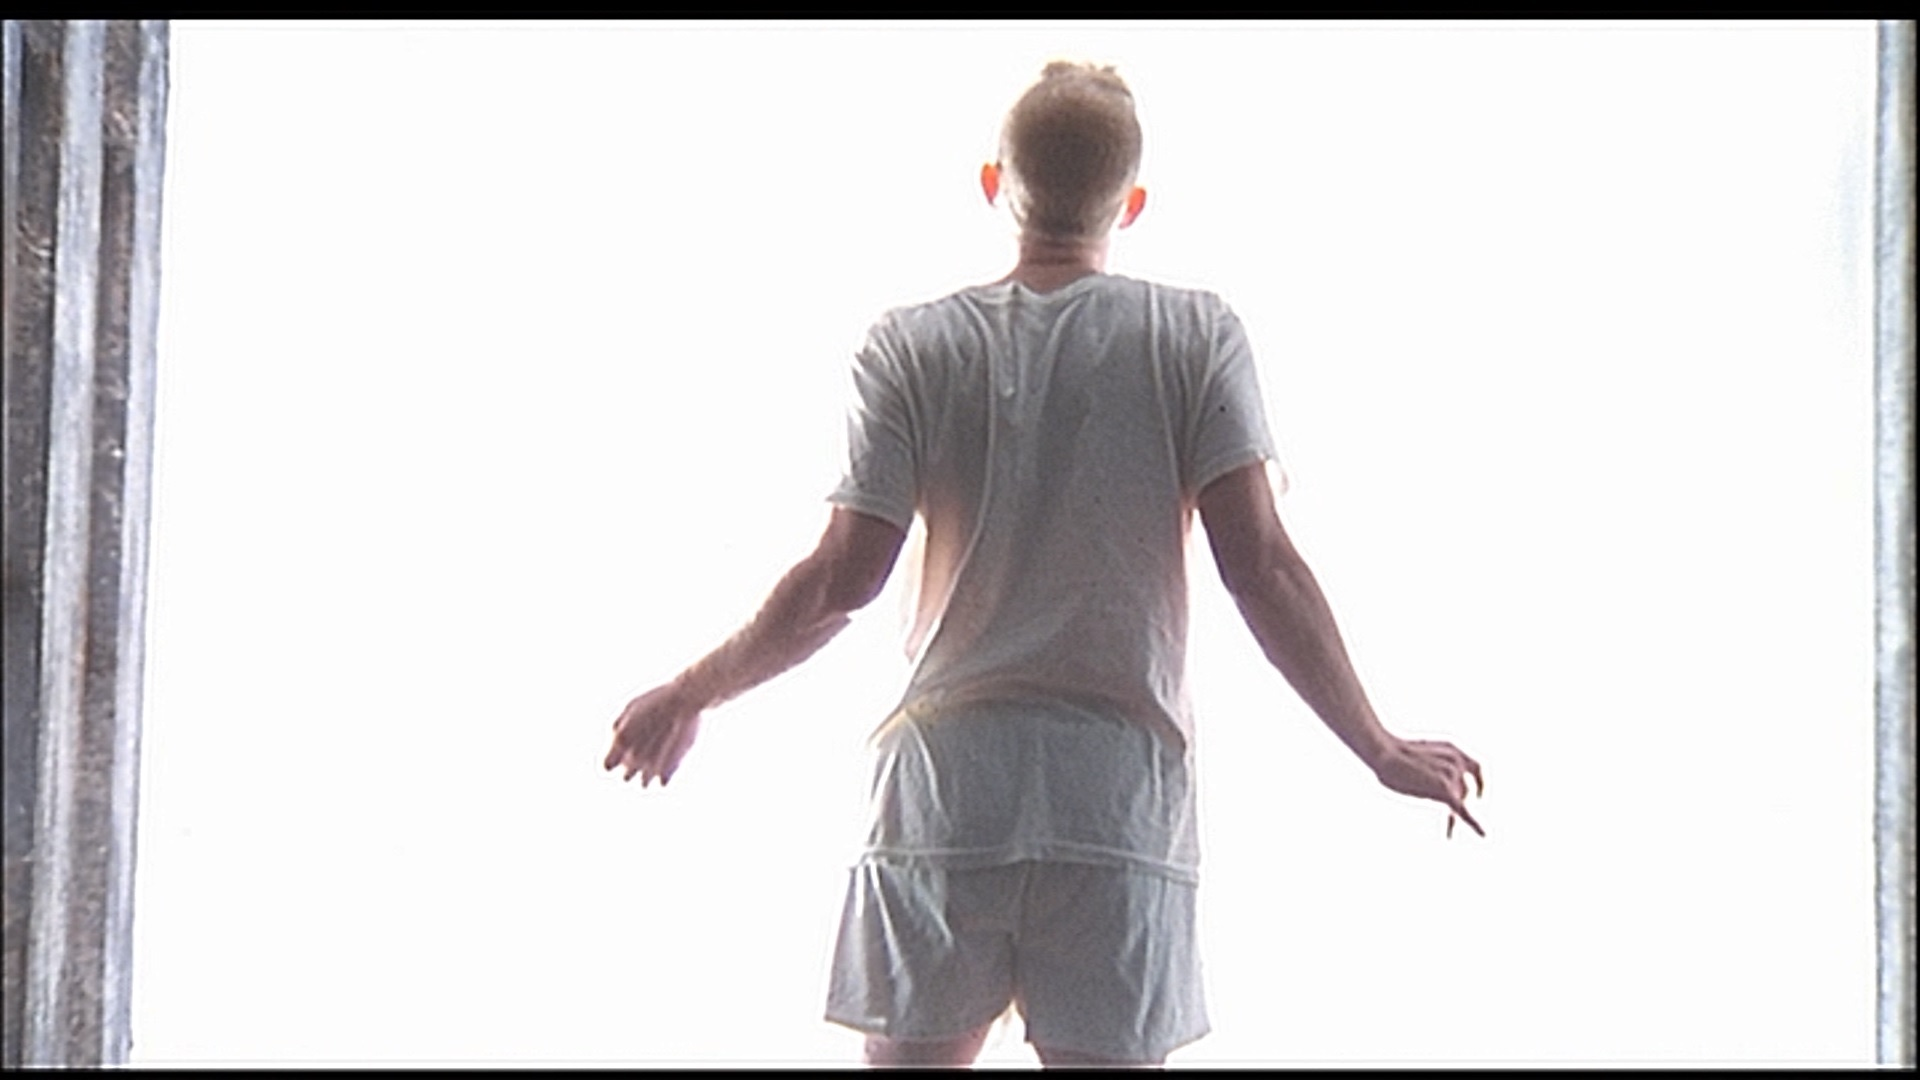
\includegraphics[scale=0.1]{光}
\caption{箱の外には光がある}
\end{minipage}
\end{tabular}
\end{figure}

この問いに答えるために、まずは、キューブの全体像を発見するに至るまでの過程をたどりなおしてみよう。キューブの内部に投げ込まれた登場人物たちは、さまざまな手段でそこにキューブの全体像の説明を見出そうとする。いわく、快楽殺人鬼が人々をこのデスゲームへと導いている。いわく、この殺人キューブの由来は政府の陰謀である。このような説明は、しかし、すでに上で述べたように、真っ向から否定されることになる。

しかし、そのような形式における説明とは別に、つまり\textbf{キューブという存在に込められた意図}や\textbf{自分たちがキューブの中にいることの理由}等の説明とは別に、\textbf{キューブの内部構造およびメカニズム}の説明もまた試みられる。手がかりは、各々の箱に取り付けられた出入り口の部分に記載されている3×3ケタの数字である。この数字の解釈を通じて、キューブを支配するルールが推測されることになる。

重要なのは、この推測がことごとく不十分なままに留まるということである。最初に推測された素数ルール------三つの数のうちいずれかが素数である場合には、その先の部屋は安全である------は、クエンティンが素数の部屋のトラップを作動させたことによって誤りであることが判明する。第二に推測されたデカルト座標のルール------三つの数はそれぞれ三次元空間における縦・横・上下方向の座標を示している------もまた、存在するはずのない座標をもつ箱を発見したことによって棄却されることになる。そして、最後のルール------箱はキューブの内部で一定時間ごとに移動しており、数字はその移動のパターンを表すものである------は、実はキューブの正しい姿を言い表しているのだが、この真理は、ある人物の助力を得ることによってのみ確かめることができる。その人物こそが、ただひとりキューブから脱出する人間であるところのカザンなのである。

そのからくりはこうである。最後に推測されたルールは非常にもっともらしかったが、箱に記載された数字から実際にその箱の位置と移動パターンを読み取るには、コンピュータ並みの計算能力が必要であった。つまり、電子機器の類を一切携行していない登場人物たちには、そのルールを実際の状況に適用することができなかったのである。そこでカザンに対して物語上の役割が与えられることになる。カザンは何らかの精神疾患を抱えていると見られ、「最後のルール」を理解することはできないが、一方で類まれな暗算能力を有しており、ルールを適用するのに必要な計算を適切に行うことができたのである。

ここに現れるのは、ルールを理解することとルールを適用することの相補性である。カザンには前者が欠けており、カザン以外の人物には後者が欠けているのだが、両者が協働することによってルールの適切な理解と適切な適用がなされ、そこでキューブの全体像がはじめて明らかになるのである。\textbf{説明の成功が、箱の統一的全体像を構成する}。説明の成功が\textbf{箱の外には箱がある}の運動を停止し、箱の外を何か別のものへと変化させるのである。ただしその成功は、カザンという例外的存在抜きにはなされえなかった。

カザンはなぜ例外的なのか。それは、彼だけがキューブの説明を試みていないからである。すなわち、\textbf{キューブという存在に込められた意図}や\textbf{自分たちがキューブの中にいることの理由}、そして\textbf{キューブの内部構造およびメカニズム}を、彼だけが問わないままにしているからである。カザンと同じくキューブからの脱出を望んでいないワースでさえ、\textbf{これは愚かな失敗である}とか\textbf{〔箱の外にあるのは〕人間の限りない愚かさである}\footnote{『CUBE』劇中のセリフより。元のセリフは"Boundless human stupidity."}という言い方で、キューブの説明を試みていた。そして実際に箱の外へと至るのは、決して説明を試みることのなかったカザンだけだった。したがって問題は、説明が試みられないゆえに説明がなされえないような状況において、キューブの絶対的外部とは何か、ということである。われわれはこの問題に対して、次のように答えなければならないだろう。すなわち、\textbf{説明の成功が箱の統一的全体像を構成する}のだから、説明がなされえないような状況においては、もはや\textbf{箱の絶対的外部は存在しえない}、と。


つまり、実のところ、説明は成功していなかったのである。実は、『CUBE』における最後のルールは、物語内では正しいルールとして扱われているが、実際には数多くのミスと矛盾を抱えている。素数であるはずの563を素数ではないとする等の計算ミスのほか、最後のルールにおける移動の規則に従うと複数の部屋の移動先が同じ場所になってしまうことなどがその例である。結局のところ、『CUBE』において、箱の説明はことごとく失敗し、箱の統一的全体像は決して構成されないのだ。箱の外の光に到達するためには、それを説明しようとしてはならない。説明の不在を通してのみ、光への接近が可能となるのである。


箱の外の光、それはあらゆる説明が失敗する地点であり、説明の不在によってのみ言い表すことのできる何かである。そういうわけで、以下のように結論しよう。\textbf{光、それは説明の失敗と不在の形象である}。光は説明されるべきものではない。光は視界を開き、さまざまなものを可視化するのだが、光そのものを見ることはできない。光は問いと答えの------疑問と説明の------可能性の条件なのだが、それ自体は問われることも、説明されることもない。つまり、結局のところ、ワースの言葉が正しかったのである。

\begin{quote}
クエンティン、あんたの言う通り、頭を垂れて、ややこしいことは言わず、目の前にあるものを見なきゃならない。
\end{quote}

\subsection*{まとめ}

「CUBE」における箱、それは、\textbf{箱の外には箱がある}の構造を有する無数の箱である。この構造の内部において、\textbf{生き延びの空間}であるところのそれぞれの箱は、相対的な生と相対的な死の配分によって互いに区別される。それと同時に、この構造の内部において、箱は\textbf{問いと答えの場所}でもある。この箱の内部では、箱の絶対的外部を目指して、さまざまな疑問と説明が繰り広げられることになる。このような構造を支えているのは、説明の失敗もしくは不在という原理であり、光はそのような原理の形象に他ならない。

\section{「すべて世はこともなし」------漫画「BOX」における「箱の中」}


\subsection{\tbaselineshift =3.0pt 箱の中には箱がある------秘密について}
諸星大二郎の中編漫画『BOX~箱の中に何かいる~』(以下「BOX」)の登場人物たちは、ある巨大な立方体型の建造物のもとへと導かれ、その中に閉じ込められてしまう。そこで彼らを待ち受けるのは、種々さまざまなパズルである。\textbf{パズルを解くと何かが起きる}------先へ進むためのドアが現れたり、体の一部が消失したりする------、そして\textbf{パズルをすべて解けば外に出られる}、という情報だけを与えられた彼らは、人体が溶けてどろどろになったような怪物たちに追われながら、箱の中をさまようことになる。


はじめに指摘しておきたいのは、彼らがそこに閉じ込められるところのこの巨大な箱は、次の二つの意味において、\textbf{箱の中には箱がある}という構造を有している、ということである。すなわち、第一に、この箱は大小さまざまな無数の箱が積み重ねられることによって構成されている。第二に、この箱は一個の「ひみつ箱」\footnote{表面や内部に仕掛けが施されており、一定の手順で操作しないと開くことのできない箱。本作冒頭で光一のもとに届く最初のパズルでもある。}であり、いくつかの部屋=箱があるシステムをなすことによって構成されている。


\begin{figure}[h]
\begin{tabular}<y>{c}
\begin{minipage}[c]{0.7\hsize}
\centering
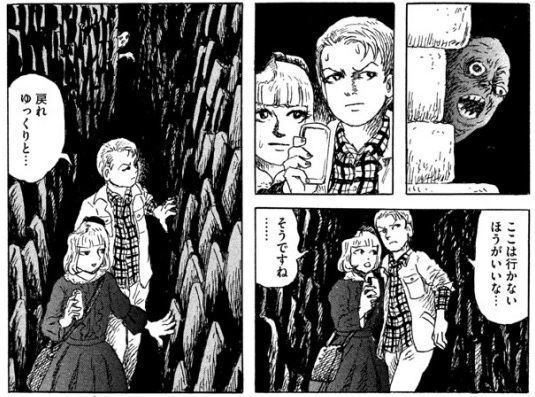
\includegraphics[scale=0.4]{箱と怪物}
\caption{箱の中には箱がある。怪物もいる。(『BOX』第一巻p. 123)}
\end{minipage}
\end{tabular}
\end{figure}

この第二の意味における\textbf{箱の中には箱がある}は、その構造のさらなる含意を開示する。つまり、この箱はそれ自体がパズルであり、それを解くことによって露わになるのは、何らかの種類の秘密なのである。ここに、「ひみつ箱」の形象を介して、箱=パズルと秘密との間の概念的な結びつきが生まれることになる。すなわち、\textbf{箱の中には秘密がある}。したがって、\textbf{パズルを解くことは、秘密を露わにすることである}。

「BOX」の登場人物たちは、それぞれが秘密を抱えている。同性愛指向やGID(性同一性障害)、手抜き工事を隠蔽した過去、息子の死に心を病んでしまった母親の存在、霊的な存在を感知する能力など、多岐にわたる秘密が、各人の箱=パズルのなかに仕舞い込まれているのである。

\begin{figure}[h]
\begin{tabular}<y>{c}
\begin{minipage}[c]{0.7\hsize}
\centering
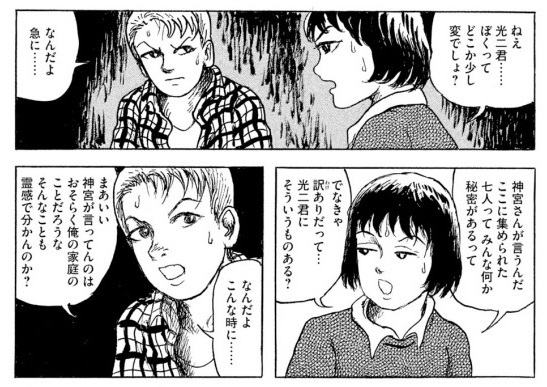
\includegraphics[scale=0.4]{秘密}
\caption{みんな秘密を抱えている(『BOX』第二巻p. 81)}
\end{minipage}
\end{tabular}
\end{figure}

さて、次なる問題は、そうした秘密が「露わになる」とはどのようなことか、ということである。「BOX」における実際の描写を参考にして考えてみよう。宅配便で送られてきた「ひみつ箱」のパズルを箱の中に入るよりも前に解いた光一は、二年前に亡くなった兄の部屋と、心を病んだ母親の頭の半分が、まるで切り取られたかのように消失していることに気付く。また、光一と同様に箱の外でパズルを解いたGIDの少年・桝田恵は、自身の男性器が同様の仕方で消失しているのを発見する。そう、\textbf{秘密は、それが露わになるとき、消失してしまう}のである。

箱の中には何かが------秘密が------入っている。しかしながら、実際に箱を開いてみると、その中は空になっている\yakuchu{\textbf{ウィトゲンシュタインの第一の箱}。「この、箱の蓋にある穴から真珠の紐が引きだされてくる視覚的イメージがあると、たしかにこう言いたくなる、「これらの粒はみんな一緒に前々から箱の中にあったに違いない。」だが、\textbf{これはひとつの仮説を述べている}のであることはすぐにわかる。もしかりに真珠の粒が次々箱の穴の所で創生してくるとしても、その[視覚的]イメージは同じであろうからである。」(ウィトゲンシュタイン『青色本』大森荘蔵訳、筑摩書房、pp. 94-95)\textbf{秘密、それはひとつの仮説である}。重要なのは、それがいずれ必然的に失敗するであろう仮説だということだ。}。この退隠の働きこそが、「BOX」における\textbf{箱の中には箱がある}という構造の特性なのである。

しかしながら、そのような消失が描写のレベルで現れるのは、\textbf{箱の外で}パズルを解いた登場人物たちにおいてのみであった。そこで、次にわれわれが取り組むべき課題は、\textbf{箱の中で}パズルを解くこと=箱を開くことにはいかなる意味があるのか、秘密の消失とは別の何かが起こっているのかそうではないのかを明らかにすることである。

\subsection{\tbaselineshift =3.0pt 箱の中には光がある------因果について}

数々の障害を乗り越え、すべてのパズルを解いた光一たちは、案内役の魔少女から箱の正体を聞かされることになる。いわく、箱の中には「物凄いもの」が潜んでおり、その「物凄いもの」は箱の中に人間を誘い込み、その一部を食べる。この箱から脱出するためには、自分の一部を差し出さなければならない。さもなければ、箱の中でお前たちを襲撃したあの怪物のような姿になって、箱の中をあてもなくさまようことになるだろう\footnote{そう、この箱もまた、光一たちがその中に入るよりもずっと前から、ある種の生き延びの空間だったのである。}。

そして、箱の最深部、「箱の中のもう一つの箱」\footnote{「BOX」第三巻p. 171.}に到達した光一たちがそこで実際に目にすることになるのは、その場を覆い尽くすほどの強烈な光であった。\textbf{箱の中には光がある}。\textbf{「物凄いもの」、箱の最大にして最深の秘密、それは光なのである}。ところで、光とは何であろうか?


\begin{figure}[h]
\begin{tabular}<y>{c}
\begin{minipage}[c]{0.65\hsize}
\centering
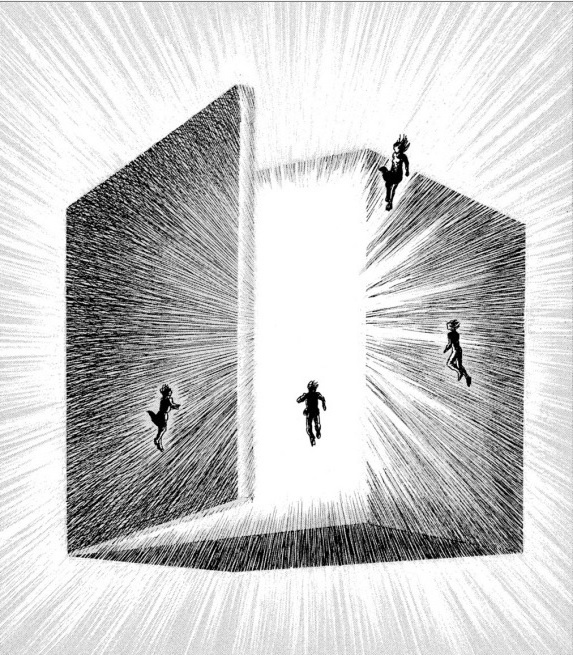
\includegraphics[clip, scale=0.3]{物凄いもの}
\caption{箱の中には光がある(『BOX』第三巻p. 203)}
\end{minipage}
\end{tabular}
\end{figure}

この問いに答えるために、まずは「物凄いもの」について作中で語られていることを見ていこう。上述したように、「物凄いもの」は箱の中の人間の一部を食べてしまうのだが、食べられることになるその「一部」とは、身体の一部分のことではない。「物凄いもの」が食べるのは、「因果」もしくは「因果の余剰」である。つまり、箱の中の人間そのものやその特徴もしくは性格、あるいはその友人や配偶者などを最初から存在しなかったことにして「因果」を書き換え、新たに生まれた因果との間の差異(「因果の余剰」)を食べるのである。

「物凄いもの」が何を要求するかは各人によって異なるのだが、ここで指摘しておかなければならない第一のことは、本作の登場人物たちは各人の秘密を要求される、ということである。箱の中の「物凄いもの」は、秘密の周囲に形成された因果を食べる。\textbf{因果は秘密の周囲に形成される}。そして第二に、「物凄いもの」が因果を書き換えるとき、秘密ははじめから存在していなかったことになるのだが、それはまた、そのような書き換え、そのような消失自体がなかったことになる、ということでもある\yakuchu{\textbf{ウィトゲンシュタインの第二の箱}。「各人が箱を一つ持っていて、その中には、われわれが「カブトムシ」と呼んでいるような何かが入っている、と仮定しよう。︙︙このとき、各人とも自分の箱の中に〔それぞれ〕ちがったものをもっていることが、当然ありえよう。ひとは、そのようなものが絶えず変化している、と想像することさえできよう。︙︙箱の中のそのものは、一般に言語ゲームの一部ではないし、また、ある何かですらない。なぜなら、その箱がからでさえありうるのだから。------いや、\textbf{箱の中のこのものを通りぬけて〈短絡させる〉ことができる}のだ。それが何であろうと、それは消え失せてしまう。」(ウィトゲンシュタイン『哲学探究』§293)\textbf{箱の中と箱の外とが短絡させられるとき、箱の中の秘密が消失するとともに、そのような消失までもが消失する。}}。箱の外への脱出に成功した光一たちは、もはや自分が何を失ったのかわからず、また何かを失ったということ自体をも忘却してしまうのである\yakuchu{「忘却してしまう」と表現したが、このことは個人の記憶の問題ではない。光一の兄の部屋および彼の遺品は実際にこの世から消え、GIDの少年は実際に女性の身体を手に入れる。「物凄いもの」へ差し出された秘密は、その痕跡を世界からまるごと消し去ってしまうのである。つまり、これはいわば世界の記憶に関する問題なのである。(ところで、ここで言及されている世界とは何だろうか。それは少なくとも、われわれがそこで生き延びているところのこの世界ではないだろう。というのも、われわれは秘密の消失の消失を漫画「BOX」におけるひとつの展開として目の当たりにしているからである。それでは、われわれとは誰なのだろう? この問いに答えるには、次の章を待たなければならない。)}。

\begin{figure}[h]
\begin{tabular}<y>{c}
\begin{minipage}[c]{0.65\hsize}
	\centering
	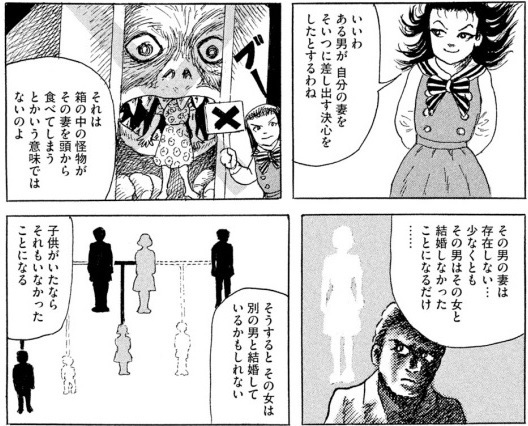
\includegraphics[clip, scale=0.4]{因果}
	\caption{すべて世はこともなし(『BOX』第三巻p. 174)}
	\end{minipage}
\end{tabular}
\end{figure}

ここに、箱の中で箱を開くことにはいかなる意味があるのか、秘密の消失とは別の何かが起こっているのかそうではないのか、という問いに対する答えがある。箱の中の箱が開かれるとき、\textbf{秘密の消失が起こるともに、そのような消失もまた消失する}のである\footnote{より正確に言えば、「物凄いもの」が秘密の消失のいかなる痕跡をも消去してしまう限り、消失の消失もまた消失し︙︙という無限の消去が起こることになる。}。「物凄いもの」は秘密および秘密が辿るはずの運命(「因果」)を食べるとともに、新たに生成する運命への変化もしくはその前後の差異(「因果の余剰」)をも食べてしまうのである。

秘密の消失の消失、それはすなわち、箱が開かれたという事実の消失である。秘密は明かされなかった。箱は開かれなかった。\textbf{箱の中で箱を開くことは、箱の外で箱を閉じたままにすることだった}。秘密および因果の消失とともに新たに生成した因果は、実際にははじめから存在していたのであって、そこに「変化」や「差異」はありえなかった。\textbf{箱は因果の化身であり、箱が閉じられたままの形で存在する限り、そこにはなめらかかつ不動の因果が存在する}。こうした一連の帰結こそが、\textbf{箱の中には光がある}の意味するものである。だから、「BOX」においてもやはり、光は説明の不在の形象である。\textbf{光において、説明されるべきことは何もない}。すべては沈黙に------沈黙に関して沈黙することに------委ねられなければならない\yakuchu{\textbf{フロイトの箱}。「︙︙小箱は女性における本質的なものを象徴し、小箱は女性そのものだ︙︙」(「小箱選びのモチーフ」p. 14)「かの老いたる者は、最初に母親からえた愛情を、女性の愛情をむなしく求めつづける。そしてこの老いたる者を腕に迎えるのは、第三の\textbf{宿命の女神、沈黙する死の女神}なのである。」(同上、p. 35. 強調は筆者。)ここに現れる沈黙、宿命、死のイメージは、不気味なものに関する彼の考察を参照するようわれわれに目配せする。「男性の神経症患者が、女性の性器はどうも不気味に感じられると語ることは多い。しかしこの不気味に感じられる性器は、人間のかつての故郷への入り口なのであり、誰もがかつて、人生の最初の時期に滞在していた場所なのである。」(「不気味なもの」p. 186)「\textbf{不気味なものとは、慣れ親しんだもの、馴染みのものであり、それが抑圧された後に回帰してきたもののことである。}」(同上、p. 187. 強調は筆者。)「この抑圧との関係を理解することによって、︙︙\textbf{不気味なものとは、隠されているべきものが外に現れたものである}という定義の意味が明らかになる。」(同上、p. 178. 強調は筆者。)沈黙に委ねられるべき親しき秘密と、その現出としての不気味なもの。\textbf{箱、それは親しき秘密の隠し処である}(あるいはむしろ、その家である([\pbox<z>{後注}f]参照))。\textbf{宿命的な死、そして死の如き宿命性は、秘密の周囲に形成される}。\textbf{秘密が、あるいはむしろ秘密に対する沈黙が現出するとき、それは不気味なものとなる。}}。

「\textbf{すべて世はこともなし}」\footnote{『BOX』第三巻p. 222.}------何も起こらず、何も消えず、\textbf{すべては日常のままである}ということ、これこそが光の意味するところのものなのである
\yakuchu{\textbf{ハイデガーの秘密}。「ひとつの秘密がそこに漲っているということ、これすらもが前面に現れてこない時に初めて、秘密は秘密なのです。」(『言葉についての対話------日本人と問う人とのあいだの』p. 129)秘密を特徴づけるのは、それに対する沈黙と、その沈黙に対するさらなる沈黙である。「とりわけ沈黙に関しては沈黙する︙︙」(同上、p. 137)ハイデガーにとって、沈黙の沈黙の下にある秘密とは、そのものとしての存在に他ならない。「存在は、単純なものとして、\textbf{秘密に充ちた[geheimnisvoll]}ものですし、押しつけがましく支配するものでない単純な近さです。」(『ヒューマニズムについて』p. 47. [ ]内および強調は筆者。)だからこそ、存在の呼び声は沈黙によって語るのである。「呼び声は、\textbf{\bou{黙止}という無気味な[unheimlich]様態}で話す。︙︙\textbf{無気味さ[Unheimlichkeit]}は、日常的には蔽いかくされているけれども、世界=内=存在の根本的様相である。」(『存在と時間』下巻pp. 115-116. 傍点はハイデガー、[ ]内および太線の強調は筆者。)\textbf{秘密が、あるいはむしろ秘密に対する沈黙が現出するとき、それは不気味なものとなる}。そしてその現出は、秘密の消失の消失へとただちに移行する。「人間は最も近いものを超えたもの〔\"Ubern\"achtes〕が最も近いものである、とさえ考えます。だがこの最も近いものよりももっと近いと同時に、\textbf{普通の考え方[gewöhnliche Denken]}にとってその最も遠いものよりももっと遠いものが近さそのもの、すなわち存在の真理なのです。」(『ヒューマニズムについて』、p. 46. [ ]内および強調は筆者。)存在は、すなわち箱の中の親しき秘密は、最も近いものよりももっと近いものであると同時に、最も遠いものよりももっと遠いものでもある。\textbf{箱の中で箱を開くことは、箱の外で箱を閉じたままにすることだった}。そしてやはり、\textbf{運命は、秘密(=存在)の周囲に形成される。}「存在は自らを思考にすでに贈り届けているのです。存在は思考の贈りもの〔\textbf{運命(Geschick)}〕として\bou{ある}のです。」(同上、p. 101. 傍点はハイデガー、太線の強調は筆者。)このようにしてわれわれは、フロイトを介して([\pbox<z>{後注e}]参照)、この秘密という通路を通じて、\textbf{ハイデガーの家}へと辿りつく。「言葉は存在の家であります。\textbf{人間は言葉という住居に住んでいる}のです。」(同上、pp. 11-12. 強調は筆者。)「思考は存在の家を建てることに従事します。存在の継ぎ目はこのような存在の家としてその都度\textbf{運命に適う}ように、人間の本質に存在の真理のなかに住むように指図します。この\textbf{住むことが《世界-内-存在》︙︙の本質です}。」(同上、p. 92. 強調は筆者。)日常性〔Gew\"ohnlichkeit〕、秘密〔Geheimnis〕、不気味なもの〔Unheimliche〕。家〔Heim〕に住む〔wohnen〕ことをめぐるこれらの隠喩系が示すのは、そこに生きる者どもの生あるいは生き延びのあり方である。次章参照。また、日常性と不気味さ(よそよそしさ)の関係については、拙論「日常性の哲学:ハーマン『怪奇実在論』の検討を通して」(『希哲』第一号)で論じている。}。

\subsubsection*{まとめ}

「BOX」における箱、それはまず、\textbf{箱の中には箱がある}の構造を有する「ひみつ箱」、すなわち\textbf{秘密の隠し処}であり、この構造の内部において、箱を開くこと=秘密を露わにすることは秘密を消失させることに等しい。とくに箱の中で箱を開く場合には、秘密が消失するだけでなく、秘密の消失それ自体が消失する。その結果として、箱は開かれず、秘密は明かされず、秘密の周囲に形成された因果はそのままにしておかれることになる(\textbf{箱は因果の化身である})。したがって、すべては日常のままであり、ここには説明されるべきものは何もない。光はそのような説明の不在もしくは失敗の原理の形象に他ならない。

\section{\tbaselineshift =4.0pt 「夢から覚めても......」------小説「箱男」における「箱」}

ここまでで確認してきたのは、あるひとつの、そして無数の箱がもつ、次の四つの属性であった。すなわち、この箱は、\textbf{生き延びの空間であり、問いと答えの場所であり、秘密の隠し処であり、因果の化身である}。最後に、安部公房の小説『箱男』の読解を通して、この四つの属性の有機的な連関を見てみよう。

\subsection{箱、それは生き延びの空間であり、秘密の隠し処である}

\begin{quotation}
これは箱男についての記録である。

ぼくは今、この記録を箱のなかで書きはじめている。頭からかぶると、すっぽり、ちょうど腰の辺まで届くダンボールの箱の中だ。

つまり、今のところ、箱男はこのぼく自身だということでもある。箱男が、箱の中で、箱男の記録をつけているというわけだ。\footnote{《ぼくの場合》『箱男』p. 7.}
\end{quotation}

安部公房の小説『箱男』は、ダンボール箱を頭からかぶり、その中で生活する「箱男」なる存在をめぐる物語である。設定上、その物語の全編は、箱男自身が手元のノートに記した「箱男の記録」だということになっている。

最初に確認しておきたいのは、\textbf{『箱男』における箱は、生き延びの空間である}ということである。ここで注意しなければならないのは、生き延びの空間は単なる生の空間と同じものではないということだ。第一章で述べたように、生き延びとは、死の危険を自身の本質的な可能性として引き受けながら生きることである。箱男にとって、箱とは「別の世界への出口」であり、単なる生とはまったく別の地点------それは死であろう------への通路なのである。

\begin{quotation}
箱はぼくにとって、やっとたどり着いた袋小路どころか、別の世界への出口のような気さえする。何処へかは知らないが、とにかく何処か、別の世界への出口︙︙。︙︙ここではっきりさせておくべきことは、要するに、\textbf{まだ死ぬ気はない}ということなのである。\footnote{《安全装置を とりあえず》『箱男』p. 27、強調は筆者。}
\end{quotation}

ただし、箱男は決して「別の世界」には至らない。箱男は死を目前にしながら、それでも\textbf{まだ死なない}。箱男は箱の外の死を覗き窓から覗きつつ、箱の中で生き延びるのである。『箱男』において、この生き延びの様態は、たとえばテレビやラジオ------それらはすべて箱に取り付けられた覗き窓である------を通してニュースを聞くことになぞらえられる。

\begin{quotation}
人はただ安心するためにニュースを聞いているだけなんだ。どんな大ニュースを聞かされたところで、聞いている人間はまだちゃんと生きているわけだからな。本当の大ニュースは、世界の終りを告げる、最後のニュースだろう。︙︙考えてみれば、ぼくが中毒にかかったのも、結局のところその最後の放送を聞きのがすまいとする焦りだったような気がする。しかし、ニュースが続いているかぎり、\textbf{まだ最後ではありません}、というお知らせなのさ。︙︙昨夜B52による本年度最大の北爆が行われました、\textbf{でもあなたはまだなんとか生きています}。ガス工事中引火して八人重軽傷、\textbf{でもあなたは無事に生きています}。物価上昇率記録更新、\textbf{でもあなたは生きつづけています}。工場廃液で湾内の魚介類全滅、\textbf{でもあなたはなんとか生きのびています}。\footnote{《書いているぼくと 書かれているぼくとの不機嫌な関係をめぐって》『箱男』p. 95、強調は筆者。}	
\end{quotation}

あらゆるニュースは「最後のニュース」でありうるが、しかしどのニュースも「最後のニュース」ではありえない。「世界の終り」はいつでも到来しうるが、しかしいずれの瞬間においても、「世界の終り」が到来することは決してない。「最後のニュース」を聞くためにニュースを聞き続けるひとびとは、まさにそのことによって、「最後のニュース」の到来をいつまでも延期させる。「世界の終り」について話し続けるひとびとは、まさにそのことによって、「世界の終り」の到来をいつまでも延期させる\yakuchu{\textbf{ラカンの話}。「実際に生活の基底をなしているものとは、男たちと女たちの関係をめぐるあらゆる事情について、︙︙ことはうまくいかないということです。それはうまくいかないのです。そして、皆がその話をしており、わたしたちの営みの大半がそれを言うことで過ぎていきます。」(『アンコール』p. 59)\textbf{日常的ディスクール}〔discours courant〕は性関係における失敗について話すことによって回転するのだが、まさにそのことによって、その失敗は覆い隠される。「ここで注意していただきたいのは、この語------\textbf{まさに}〔juste〕------によって導入される変化です。この\textbf{まさに}〔juste〕、\textbf{まさしく}〔justement〕は、\textbf{ぎりぎりの}〔tout juste〕、\textbf{かろうじて成功した}〔tout juste r\'eussi〕ということであり、失敗したものの裏側を示しています------それは\textbf{かろうじて}〔tout juste〕成功します。」(同上、p. 114)\textbf{箱は、性的関係を失敗させる障害であるとともに、その関係をかろうじて成功させる契機でもある}。\textbf{フロイトの箱}を思い出そう。フロイトにとって、箱とは死の女神であり、箱の中の親しき秘密とは、その性器なのであった([\pbox<z>{後注e}]参照)。\textbf{箱の中には女性がいる}。箱男は覗き窓から女性を覗くことに徹することによって女性との直接的な関係を断つのだが、まさにそのことによって、女性との性的な関係を保つことにかろうじて成功するのである。}。箱が表しているのはこのような形式における------「まだ生きている」という形式における------生き延びのあり方なのである。

また、\textbf{『箱男』における箱は、秘密の隠し処でもある}。『箱男』における秘密とは何か。それは箱の中の人物そのものである。このことを確かめるには、まずは箱男の匿名性について語らなければならない。

箱男は、次の二重の意味において匿名的である。第一に、箱男はホームレスのような周辺的存在とも異なる、独特の意味における不可視の存在であるという点で、匿名的な存在である。

\begin{quotation}
統計があるわけではないが、全国各地にはかなりの数の箱男が身をひそめているらしい痕跡がある。そのくせどこかで箱男が話題にされたという話は、まだ聞いたこともない。どうやら世間は、箱男について、固く口をつぐんだままにしておくつもりらしいのだ。︙︙箱男が目立ちにくいのは、たしかである。︙︙だが目立たないのと、見えないのとは違う。︙︙君だって、目撃したことくらいはあるに違いない。しかしそれを認めたくない気持も同じくらいよくわかる。見て見ぬふりは、なにも君だけとは限らないのだ。\footnote{《たとえばAの場合》『箱男』pp. 13-14.}
\end{quotation}

\begin{quotation}
「箱男なんて、気にしなければ、風やほこりみたいなものだよ。︙︙それにしても驚いたね。あれほど近くに写っているからには、目撃しなかったはずがない。だのにさっぱり記憶がない。見えてもいないのに、見えたような気がするのが幽霊なら、ちょうど正反対の存在だな。︙︙」\footnote{《書いているぼくと 書かれているぼくとの不機嫌な関係をめぐって》『箱男』pp. 100-101.}	
\end{quotation}

箱男のこの不可視性は、社会から排除されていることというよりもむしろ、(風やほこりのように)社会にあまりにもよく馴染んでいることに由来する。箱男は、それがあまりにも日常的な存在であるがゆえに、誰にも見られることがないのである。

\begin{quotation}
雑踏のなかで、箱男らしい時をすごすためには、どうしても街に馴れきってしまわなければならない。馴れてしまえば、時間は箱男を中心に、同心円を描いてまわりはじめるのだ。\footnote{《ここに再び そして最後の挿入文》『箱男』p. 173.}
\end{quotation}

第二に、箱男は、箱の中に誰が入っているのか誰にもわからないという点で匿名的である。この第二の意味における匿名性は、第一の意味における匿名性によって、より強固な形で実現される。『箱男』の直前に発表された短編「箱男 予告編」における箱男襲撃の場面は、このことの好例である\footnote{安部公房は長編作品を執筆する際、しばしばその原型となる短編小説をあらかじめ発表する。『砂の女』に対する「チチンデラ ヤパナ」、『燃えつきた地図』に対する「カーブの向う」、『方舟さくら丸』に対する「ユープケッチャ」などがその例である。『壁男』の場合、「物語とは」「ところで君は」「これはある職業的関係によって」「あるいはAの場合」「箱男 予告編」「箱男 予告編 その2」が雑誌『波』上に先んじて発表され、「箱男 予告編」を除くすべての作品が改稿・改題ののちそれぞれ『箱男』の中の一章として収録されている。}。ある男が箱男に襲いかかり、後にはひとりの箱男と一体の死体が残される。さて、誰が殺され、誰が生き残ったのか。

\begin{quotation}
仮に、その切通しの下の死体を、失敗した襲撃者だとすれば、いま立去って行った箱男は、縫いぐるみの鰐で逆襲に成功したBだということになり、べつに問題はなさそうだ。

︙︙では、反対に、殺されたのがBの方だった場合は、どういう事になるのだろう。あいにく、事情はまったく変らないのだ。原因不明の事故による、ごくありふれた変死体。前には彼を守ってくれた同じ条件が、今度は彼を見殺しにする。箱男に化けた襲撃者は、一見して箱男だというだけで、無事容疑者リストから除外してもらえるのだ。\footnote{「箱男 予告編」p. 395}
\end{quotation}

そう、誰であっても「事情はまったく変らない」のである。箱男の不可視性という「条件」のために、箱の中に誰が入っているのかということは、そもそも問題にはならないのだ。

このように、箱男は二重の意味で匿名的な存在であり、特にその第二の意味において、箱の中身はそもそも問題にされることがない。それにもかかわらず\textbf{箱の中には秘密がある}のだとすれば、そして\textbf{秘密とは箱の中の人物そのものなのだ}とすれば、それはなぜか。鍵は、箱男が記す「箱男の記録」、すなわち『箱男』の文章そのものであるところのノートにある。箱男は匿名的な存在になるために、言い換えれば自らの不在証明を行うために箱の中に入るのだが、それにもかかわらず、自身の存在を証明する「安全装置」として、ノートを書くのである。

\begin{quotation}
そこでせめてもの安全装置。もしも万一のことがあった場合、ぼくはこのノートを証拠物件として残しておくつもりである。どんな死に方をしようと、ぼくには自殺の意志など少しもなかった。ぼくが死ねば、間違っても自殺なんかではなく、絶対に他殺なのである。\footnote{《安全装置を とりあえず》『箱男』p. 25.}
\end{quotation}

箱男は、ノートを所有することによって自らの完全な匿名化を回避し、それと同時に、箱の中に秘密を------自らの非匿名的な、秘匿された存在を------抱えることになる。箱男は箱の中で、かけがえのない自己自身として生き延びるのである\footnote{事前に発表された短編作品の中で「箱男 予告編」だけが『箱男』に組み込まれることがなかったのは、あるいはこの理由のためなのかもしれない。}。ここに示されるのは、生き延びと秘密のあいだの関係である。\textbf{生き延びること、それは自己自身として------自己の存在という秘密を抱えて------生きることである}。

さて、われわれはここまで、『箱男』の前半部を中心にその読解を行ってきた。しかしながら、『箱男』における中心的な問題は、むしろその後半部に属している。次の節では、『箱男』後半部の読解を通じて、箱の諸属性の関係のさらなる検討を行おう。


\subsection{箱、それは問いと答えの場所であり、因果の化身である}

『箱男』の後半部、より具体的には《書いているぼくと 書かれているぼくとの不機嫌な関係をめぐって》と題された章以降の部分において問題になるのは、ノートの記述者または所有者の身分の問題である。すでに述べたように、ノートは箱の中の秘密=自己の存在を証明する「安全装置」であり、その意味でいわば自己の自己らしさの源泉なのだが、この章では、そのノートの所有権をめぐる「ぼく」と「医者」の間の争いが記述される。

\begin{quotation}
「︙︙とにかく、君に箱から出る気がないことだけは、これではっきりしたわけだ。」
	
「箱は始末して来たと言っただろう。」
	
「︙︙それじゃ聞くけど、君はいまこの瞬間に、何処で、何をしているんだい?」
	
「あんたの見ているとおりさ。ここで、あんたと、喋くっているよ。」
	
「なるほど︙︙すると、\textbf{このノートは、何処で誰が書いていることになるのかな?} 誰かが、箱の中で、海岸の脱衣場の裸電球をたよりに書いていたんじゃなかったっけ?」\footnote{《書いているぼくと 書かれているぼくとの不機嫌な関係をめぐって》『箱男』p. 118、強調は筆者。}	
\end{quotation}

この場面では、「ぼく」は箱の外に出て「医者」と対面しているのだが、問題は、この場面を記述するノートが、設定上、箱の中の「ぼく」の手によって書かれたものだということになっている、ということである。ここには次の二通りの可能性がある。1、「ぼく」は箱の外には出ていない。2、「ぼく」はノートの記述者あるいは所有者ではない。重要なのは、この二通りの可能性の間で、どちらが正しいのかを決定することができないということだ。

\begin{quotation}
「そうだろう、このノートの筆者を、君だと決めてかかる必要なんかどこにもないんだ。君以外の誰かが筆者であっても、いっこうに差支えないわけだからな。」

「言いがかりはよしてくれ。現にぼくはこうして書いている。海の臭いが立ち込めている、暗い海岸だ。︙︙もし今ここで、ぼくが書きやめたら、次の一字一句だって、出て来はしないんだ。」

「︙︙と、誰か別の人間が、何処か別の場所で書いているのかもしれない。」

「誰が?」

「たとえば、ぼくだっていい。」\footnote{《書いているぼくと 書かれているぼくとの不機嫌な関係をめぐって》『箱男』pp. 124-125.}
\end{quotation}

この決定不可能性の領域を利用して、「医者」はノートの所有権を「ぼく」から奪い取ろうとする。実際、この章の次の章である《供述書》は、「ぼく」ではなく「医者」の筆によるものである。

このようにして、「ぼく」はノートの所有権を喪失し(あるいはむしろ、それを見失い)、自己がかけがえのない自己自身として生き延びていることを確信できない状況に置かれることになる。

\begin{quotation}
ぼくが、ぼくでないかもしれないというのに、そうまでしてぼくを生きのびさせる必要がどこにあるのだろう。︙︙たしかに\textbf{ぼくがまだ生きのびているという証拠は、どこにもない}のである。\footnote{《書いているぼくと 書かれているぼくとの不機嫌な関係をめぐって》『箱男』p. 131、強調は筆者。}
\end{quotation}

《供述書》以降の章においては、書き手が代わる代わる交代することになるのだが、それぞれの書き手による記述の間には、明白な矛盾や物理的に困難な状況をいくつも見て取ることができる。つまり、ここに現れている事態は、それぞれの書き手が同じ現実をそれぞれの仕方で記述しているといったものではなく、ある書き手の記述の全体が(幻覚を見てそれを記述した等)信頼できないものであったり、またそれが別の書き手によって編集・創作・偽造されていたりする、というものなのである。『箱男』はこのような仕方で、ノートの所有者=書き手の身分を攪乱する。その結果として、箱の中の秘密は失われることになる。ここで、箱とはもちろん小説の記述それ自体のことであり、箱の中の秘密とは、それが示す固有の自己のことである。

しかし、果たして、その攪乱は十分に成功していると言えるだろうか。『箱男』において、書き手は決して決定されず、箱の中の秘密=固有の自己は決定的なまでに失われている、と言えるだろうか。\textbf{言えない}、という点が重要なのである。というのも、事実としてわれわれは『箱男』を、\textbf{安部公房という著者の手による長編小説}として自然に受け取ることができるからだ。小説内でどれだけ実験的な試みがなされているとしても(たとえば安部公房自身が作中に登場するのだとしても\footnote{《供述書》の筆者の誕生日であるとされる「三月七日」(《供述書》『箱男』p. 132)は、安部公房自身の誕生日と一致する。})、われわれはそれを安部公房による試みとして受け取るだろう。\textbf{そこに安部公房の存在証明を見つけることがまったくできないとしても}、である。

つまり、小説という箱の外に出て、その書き手としての身分を奪うことは(「医者」は、自分が存在する場面がノートの記述の一部であることを指摘することによって、その場面の外へと脱出し、書き手としての身分を奪取する)、結局のところ、別の箱の中に入ることなのである(「医者」はしかし、安部公房の小説『箱男』の登場人物の一人に他ならない)。\textbf{箱の外には箱がある}。だから、箱の「絶対的外部」へと脱出し、そこに存在する書き手の身分を奪うことはできない。\textbf{箱の外には光がある}。

\begin{quotation}
箱男は、何度繰り返して夢から覚めても、けっきょく箱男のままでいるしかないらしいのだ。\footnote{《それから何度かぼくは居眠りをした》『箱男』p. 52.}	
\end{quotation}

また、書き手の身分を問い、攪乱することができるのは、小説という箱の内部においてのみである。つまり、安部公房という秘密の中の秘密に関して沈黙することによってのみ、箱の中の秘密に関する問いと答えの可能性が開かれるのである。\textbf{箱の中には箱がある}。そして、\textbf{箱の中には光がある}。

\begin{quotation}
じっさい箱というやつは、見掛けはまったく単純なただの直方体にすぎないが、いったん内側から眺めると、百の知恵の輪をつなぎ合わせたような迷路なのだ。もがけば、もがくほど、箱は体から生え出たもう一枚の外皮のように、その迷路に新しい節をつくって、ますます中の仕組みをもつれさせてしまう。\footnote{《︙︙︙︙︙︙︙︙︙》『箱男』p. 212.}	
\end{quotation}

\textbf{箱は、だから、問いと答えの場所である}。箱の内部における問いと答えは、決定的な真相------秘密の中の秘密------の周りで、その真相を執拗に避けながら、なめらかな因果を形成し、それを真相の説明とするだろう。

\begin{quotation}
物語とは、因果律によって世界を梱包してみせる思考のゲームである。\footnote{「〈物語とは〉」p. 111}

不都合なのは、筋が通らないことよりも、むしろなめらかに通りすぎている点だろう。真相というものは、欠落部分の多い嵌め絵のように、もっと切々で、飛躍だらけなものであるはずだ。\footnote{《書いているぼくと 書かれているぼくとの不機嫌な関係をめぐって》『箱男』p. 131.}
\end{quotation}

その意味で、\textbf{箱は、因果の化身である}。箱がそこに閉じられたままの形で存在する限り、秘密の周囲に形成された因果はどこまでもなめらかなままである。たしかに、一度箱の中の箱が開けば、すなわち秘密の中の秘密が露わにされれば、因果は消失するだろう。しかしその際には、箱の中がもうひとつの箱であることによって、すなわち小説の書き手の沈黙に委ねられた事実的な存在によって、因果の消失それ自体が消失し、いずれ必然的に失敗するであろう仮説とその周囲のなめらかかつ不動の因果とが、その世界をすでに埋め尽くしているであろう\footnote{ここに、「われわれとは誰なのか」という問い([\pbox<z>{後注e}]参照)に対する答えがある。われわれとは、小説の書き手と同じ世界に住まう存在のことである。われわれは、この世界の内部において、「BOX」や『箱男』における秘密の消失の消失を目の当たりにすることができる。ただしその把握は、あくまで誤解に基づくものでしかありえない。なぜなら、われわれはわれわれの世界に住まう限り、秘密の消失の消失をそのものとして言い表すことができないからである。秘密は沈黙に委ねられなければならない。とりわけ沈黙に関しては沈黙しなければならない。だから、実際のところ、われわれはわれわれが抱えている根源的な秘密を、決して把握することができない。}。したがって、\textbf{すべては日常のままである}。

\subsection*{まとめ}

\textbf{『箱男』における箱、それは生き延びの空間であり、秘密の隠し処であり、問いと答えの場所であり、因果の化身である。}つまり、箱の中の秘密としての固有の自己の存在がその中で生き延びる空間であるとともに、その自己の存在を疑問と説明の領域へと呼び出す契機を含む場所である。ただし、そのような呼び出しは(あるいは、その契機さえも)、決してそのものとして現れることはない。\textbf{箱の外には箱がある}と\textbf{箱の中には箱がある}の二つの構造によって、秘密の現出=消失はただちに消失してしまうのである。後には、なめらかかつ不動の因果と、その中心に位置する秘密とが、手つかずのまま残る(もしくは、はじめから残っていた)。つまり、すべては日常のままなのである。

\section{結論}

われわれは「CUBE」「BOX」「箱男」の読解を通じて、以下の四つの属性を持つ箱のさまざまな様態を記述してきた。その四つの属性とはすなわち、\textbf{生き延びの空間、問いと答えの場所、秘密の隠し処、因果の化身}である。これらの属性のそれぞれは、箱が持つ\textbf{箱の外には箱がある}および\textbf{箱の中には箱がある}という二種の構造------いわば、箱の内部と外部の無限の連鎖------に支えられていた。しかしながら、同時に、その構造それ自体の基盤として、\textbf{箱の外には光がある}および\textbf{箱の中には光がある}という原理が存立していた。光は説明の失敗もしくは不在の原理であり、このような原理によって、箱の無限の連鎖は停止し、秘密の中の秘密としての固有の自己の生き延びや、その周囲に形成されるなめらかな因果およびさまざまな疑問と説明の可能性が開かれるのである。しかしながら、箱の中で生き延びる存在は、その光に到達することも、それを言い表すこともできない。光は説明されるべきものではない。実は、われわれがわれわれの世界において日常を生き延びる仕方もまた、そのようなものなのである\footnote{注\rensuji{28}参照。}。
\clearpage
\theendnotes
\begin{thebibliography}{99}
{\small
\subsection*{一次資料}
\bibitem{CUBE}ヴィンチェンゾ・ナタリ監督『CUBE ファイナル・エディション』ポニーキャニオン、一九九九年。
\bibitem{BOX}諸星大二郎『BOX~箱の中に何かいる~』全三巻、講談社、二〇一六--七年。
\bibitem{箱男}安部公房『箱男』新潮社、一九八二年。
\bibitem{物語とは}------「〈物語とは〉------周辺飛行1」、『安部公房全集23』所収、新潮社、一九九九年。
\bibitem{予告編}------「箱男 予告編------周辺飛行13」、『安部公房全集23』所収、新潮社、一九九九年。
\subsection*{その他}
\bibitem{MS}アルベール・カミュ『シーシュポスの神話』新潮社、一九六九年。
\bibitem{MK}ジークムント・フロイト「小箱選びのモチーフ」中山元訳、『ドストエフスキーと父親殺し/不気味なもの』所収、光文社、二〇一一年。
\bibitem{Un}------「不気味なもの」中山元訳、『ドストエフスキーと父親殺し/不気味なもの』所収、光文社、二〇一一年。
\bibitem{SZ}マルティン・ハイデッガー『存在と時間』上下巻、細谷貞雄訳、筑摩書房、一九九四年。
\bibitem{UH}------『ヒューマニズムについて』佐々木一義訳、理想社、一九七四年。
\bibitem{GS}------『言葉についての対話:日本人と問う人とのあいだの』高田珠樹訳、平凡社、二〇〇〇年。
\bibitem{EC}ジャック・ラカン『アンコール』藤田博史・片山文保訳、講談社、二〇一九年。
\bibitem{BB}ルートヴィヒ・ウィトゲンシュタイン『青色本』大森荘蔵訳、筑摩書房、二〇一〇年。
\bibitem{PU}------『哲学探究』藤本隆志訳、大修館書店、一九七六年。
\bibitem{suki}舞城王太郎「ニオモ」『好き好き大好き超愛してる。』所収、講談社、二〇〇八年。
}
\end{thebibliography}

\end{document}
